\documentclass{report}
\usepackage[T1]{fontenc}
\usepackage[a4paper,left=2cm,right=2cm,top=2cm,bottom=2cm]{geometry}

\usepackage{amsmath}
\usepackage{amssymb}
\usepackage{array}
\usepackage{enumitem}
\usepackage{epsfig}
\usepackage{fancyhdr}
\usepackage{graphicx}
\usepackage{listings}
\usepackage{multicol}
\usepackage{tikz}
\usepackage{upquote}
\usepackage{xparse}
\usepackage{zref-abspage}
\usepackage{zref-savepos}
\usepackage{zref-user}

% PDF metadata.
\usepackage[
    pdftex,
    hidelinks,
    pdftitle={CSE Cracks 20XX - Regular Expressions -- Answer Key},
    pdfcreator={Quiz Generator},
    pdfkeywords={Version: 5b1c7da4}
]{hyperref}

% Remove paragraph indentation.
\setlength{\parindent}{0pt}

\DeclareMathOperator*{\argmax}{arg\,max}
\DeclareMathOperator*{\argmin}{arg\,min}

\usetikzlibrary{calc}

% Make a checkbox for multiple choice questions and record the bounding boxes to the positions file.
% Args: {text}[type identifier][question id][part id][answer id]
\newcommand{\radio}[5][none]{%
    \begin{tikzpicture}[color=black, line width=0.4mm]
        \fill[transparent] (0mm,0mm)
            node {\zsavepos{#3-#4-#5-ll}}
            rectangle (6mm,6mm)
            node {\zsavepos{#3-#4-#5-ur}};
        \draw [fill=#1] (3mm,3mm)
            circle (2.5mm);
    \end{tikzpicture} %
    \write\positionOutput{%
        #3,#4,#5,%
        #2,%
        \arabic{abspage},%
        \zposx{#3-#4-#5-ll}sp,\zposy{#3-#4-#5-ll}sp,%
        \zposx{#3-#4-#5-ur}sp,\zposy{#3-#4-#5-ur}sp,%
        \the\paperwidth,\the\paperheight,%
        bottom-left%
    } \relax %
}

% Make a checkbox and record the bounding boxes to the positions file.
% Args: {fill color}[type identifier][question id][part id][answer id]
\newcommand{\checkbox}[5][none]{%
    \begin{tikzpicture}[color=black, line width=0.4mm]
        \fill[transparent] (0mm,0mm)
            node {\zsavepos{#3-#4-#5-ll}}
            rectangle (6mm,6mm)
            node {\zsavepos{#3-#4-#5-ur}};
        \draw [fill=#1] (0.5mm,0.5mm)
            rectangle (5.5mm,5.5mm);
    \end{tikzpicture} %
    \write\positionOutput{%
        #3,#4,#5,%
        #2,%
        \arabic{abspage},%
        \zposx{#3-#4-#5-ll}sp,\zposy{#3-#4-#5-ll}sp,%
        \zposx{#3-#4-#5-ur}sp,\zposy{#3-#4-#5-ur}sp,%
        \the\paperwidth,\the\paperheight,%
        bottom-left%
    } \relax %
}

% Make a general large answer box and record the bounding boxes to the positions file.
% Args: {text}[height][length modifier (modifies \textwidth)][type identifier][question id][part id][answer id]
\NewDocumentCommand{\bigAnswerBox} { O{} m m m m m m }{%
    \begin{tikzpicture}[color=black, line width=0.4mm]
        \fill[transparent] (0mm, 0mm)
            node {\zsavepos{#5-#6-#7-ll}}
            rectangle (#3 \textwidth, #2)
            node {\zsavepos{#5-#6-#7-ur}};
        \draw (0.5mm,0.5mm)
            rectangle (#3 \textwidth - 0.5mm, #2 - 0.5mm)
            node[midway, red] {#1};
    \end{tikzpicture} %
    \write\positionOutput{%
        #5,#6,#7,%
        #4,%
        \arabic{abspage},%
        \zposx{#5-#6-#7-ll}sp,\zposy{#5-#6-#7-ll}sp,%
        \zposx{#5-#6-#7-ur}sp,\zposy{#5-#6-#7-ur}sp,%
        \the\paperwidth,\the\paperheight,%
        bottom-left%
    } \relax %
}

% Make a general answer box and record the bounding boxes to the positions file.
% Args: {text}[type identifier][question id][part id][answer id]
\NewDocumentCommand{\smallAnswerBox} { O{} m m m m }{%
    \begin{tikzpicture}[color=black, line width=0.4mm]
        \fill[transparent] (0cm, 0cm)
            node {\zsavepos{#3-#4-#5-ll}}
            rectangle (1cm, 1cm)
            node {\zsavepos{#3-#4-#5-ur}};
        \draw (0.5mm,0.5mm)
            rectangle (0.95cm, 0.95cm)
            node[midway, red] {#1};
    \end{tikzpicture} %
    \write\positionOutput{%
        #3,#4,#5,%
        #2,%
        \arabic{abspage},%
        \zposx{#3-#4-#5-ll}sp,\zposy{#3-#4-#5-ll}sp,%
        \zposx{#3-#4-#5-ur}sp,\zposy{#3-#4-#5-ur}sp,%
        \the\paperwidth,\the\paperheight,%
        bottom-left%
    } \relax %
}

\newdimen\remainingheight
\newcommand*{\calcremainingheight}{%
    \ifdim\pagegoal=\maxdimen
        \remainingheight\dimexpr\textheight-0.4pt\relax
    \else
        \remainingheight\dimexpr\pagegoal-\pagetotal-\lineskip-0.4pt\relax
    \fi
}

% Write positions to <job>.pos .
\newwrite\positionOutput
\openout\positionOutput=\jobname.pos\relax

% Code display settings.
\lstset{
    basicstyle=\ttfamily\small,
    columns=fixed,
    fontadjust=true,
    basewidth=0.5em,
    showspaces=false,
    showstringspaces=false,
    showtabs=false,
    frame=single,
    tabsize=4,
    breaklines=true,
    breakatwhitespace=false,
}

% Clear headers and footers for the first page.
\pagestyle{fancy}
\fancyhead{}
\renewcommand{\headrulewidth}{0mm}
\fancyfoot{}
\renewcommand{\footrulewidth}{0mm}

\begin{document}

\centerline{\Large CSE Cracks \hfill Regular Expressions -- Answer Key \hfill 20XX}
\vspace{0.2cm}

\hrule

\vspace{0.5cm}

\begin{tabular}{ m{2.0cm} m{5cm} }
    Name: & \bigAnswerBox[Answer Key]{4em}{0.80}{name}{name}{0}{0} \\
\end{tabular}

\begin{tabular}{ m{2.0cm} m{5cm} }
    Student ID: & \bigAnswerBox[Answer Key]{4em}{0.80}{id}{email}{0}{0} \\
\end{tabular}

\hrule

\vspace{1.0cm}

This quiz is open note, open book, and open world. Assume all regular expressions are done in Python using the \verb|re| standard library. Good luck!

\vspace{1.0cm}

By signing below, I acknowledge that I have neither given nor received inappropriate help on this exam, and have abided by the letter and spirit of the University of California, Santa Cruz Code of Academic Integrity while taking this exam.

\vspace{0.25cm}

\begin{tabular}{ m{2.0cm} m{5cm} }
    Signature: & \bigAnswerBox[Answer Key]{4em}{0.80}{signature}{signature}{0}{0} \\
\end{tabular}

\vspace{0.25cm}

Fill in the box below if you believe your exam may require manual grading,
e.g., you crossed out answers or needed space outside a designated answer box. \\
\begin{tabular}{ m{10mm} l }
    \checkbox{manual_grading}{manual_grading}{0}{0} & My exam may require manual grading. \\
\end{tabular}

\newpage

% Set headers and footers.
\pagestyle{fancy}
\fancyhead{}
\fancyhead[L]{CSE Cracks}
\fancyhead[C]{Regular Expressions -- Answer Key}
\fancyhead[R]{20XX}
\renewcommand{\headrulewidth}{0.1mm}
\fancyfoot{}
\fancyfoot[R]{\thepage}
\fancyfoot[L]{Version: 5b1c7da4}
\renewcommand{\footrulewidth}{0.1mm}

%%% BEGIN Group {0 -- Ice Breaker} %%%


%%% BEGIN Question {1 -- Ice Breaker} %%%

\begin{minipage}{\textwidth}
    \noindent
        \textbf{Question 1} [Ice Breaker] (5 Points)
    \vspace{0.25cm}

    \noindent
    Taking inspiration from the XKCD comic below,
how would you save the day using regular expressions?

\begin{center}

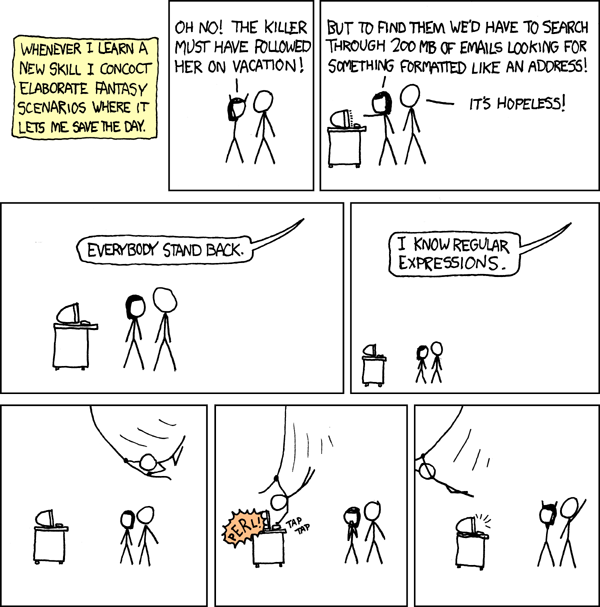
\includegraphics[width=1.00\textwidth]{images/Regular Expressions -- Answer Key/000.png}

\end{center}

    \vspace{0.25cm}

    Place your answer within the boxed region below.

        \vspace{0.25cm}


        \begin{center}

    \bigAnswerBox[detective work]{4em}{1.0}{short_answer}{0.0}{0}{0}

        \end{center}
\end{minipage}

%%% END Question {1 -- Ice Breaker} %%%



%%% END Group {0 -- Ice Breaker} %%%

\vspace{1.0cm}

%%% BEGIN Group {1 -- Regular Expression in Programming Languages} %%%


%%% BEGIN Question {2 -- Regular Expression in Programming Languages} %%%

\begin{minipage}{\textwidth}
    \noindent
        \textbf{Question 2} [Regular Expression in Programming Languages] (5 Points)
    \vspace{0.25cm}

    \noindent
    Regular expressions are implemented as either a core feature or in the standard library of almost every major programming language.

    \vspace{0.25cm}

    Fill in the circle that corresponds to your answer.

        \vspace{0.25cm}



        \begin{center}

        \begin{tabular}{ >{\centering\arraybackslash}m{0.06\textwidth} m{0.8\textwidth} }
                \radio[red]{true_false}{1.0}{0}{1.0.0}
                    & True \\
                \radio{true_false}{1.0}{0}{1.0.1}
                    & False \\
        \end{tabular}

        \end{center}
\end{minipage}

%%% END Question {2 -- Regular Expression in Programming Languages} %%%



%%% END Group {1 -- Regular Expression in Programming Languages} %%%

\vspace{1.0cm}

%%% BEGIN Group {2 -- Regular Expression Vocabulary} %%%


%%% BEGIN Question {3 -- Regular Expression Vocabulary} %%%

\begin{minipage}{\textwidth}
    \noindent
        \textbf{Question 3} [Regular Expression Vocabulary] (20 Points)
    \vspace{0.25cm}

    \noindent
    Match the following terms to their corresponding definitions.

    \vspace{0.25cm}

    Fill in the each box on the left with a letter from the right.

        \vspace{0.25cm}

    \begin{tabular}{ >{\centering\arraybackslash}m{0.08\textwidth} m{0.17\textwidth} }
                \smallAnswerBox[B]{matching}{2.0}{2.0.1}{0} & Back Reference \\
                \smallAnswerBox[E]{matching}{2.0}{2.0.2}{0} & Anchor \\
                \smallAnswerBox[K]{matching}{2.0}{2.0.3}{0} & Kleene Star \\
                \smallAnswerBox[J]{matching}{2.0}{2.0.4}{0} & Disjunction \\
                \smallAnswerBox[I]{matching}{2.0}{2.0.5}{0} & Character Class \\
                \smallAnswerBox[D]{matching}{2.0}{2.0.6}{0} & Group \\
                \smallAnswerBox[C]{matching}{2.0}{2.0.7}{0} & Word Boundary \\
    \end{tabular}
    \begin{tabular}{ >{\centering\arraybackslash}m{0.05\textwidth} m{0.60\textwidth} }
            A. & An operator that allows us to select both of two options. \\[0.5cm]
            B. & A special character that allows us to invoke a previous group. \\[0.5cm]
            C. & The empty string between (\verb|[\W^]| and \verb|\w|) or between (\verb|\w| and \verb|[\W$]|). \\[0.5cm]
            D. & A collection of character that can be treated as a single unit. \\[0.5cm]
            E. & A special character that can be used to match the beginning or end of a line. \\[0.5cm]
            F. & The set of all alphanumeric characters and underscore. \\[0.5cm]
            G. & A repetition operator that matches the range $ [1, infinity] $. \\[0.5cm]
            H. & All digits. \\[0.5cm]
            I. & A set of character where any single member of the group can be matched. \\[0.5cm]
            J. & An operator that allows us to select one of two options. \\[0.5cm]
            K. & A repetition operator that matches the range $ [0, infinity] $. \\[0.5cm]
    \end{tabular}
\end{minipage}

%%% END Question {3 -- Regular Expression Vocabulary} %%%



%%% END Group {2 -- Regular Expression Vocabulary} %%%

\vspace{1.0cm}

%%% BEGIN Group {3 -- Basic Regular Expressions} %%%


%%% BEGIN Question {4 -- Basic Regular Expressions} %%%

\begin{minipage}{\textwidth}
    \noindent
        \textbf{Question 4} [Basic Regular Expressions] (5 Points)
    \vspace{0.25cm}

    \noindent
    Which of the following regular expressions would be best to match a 10-digit phone number formatted as: '123 456-7890'. (Assume any stretch of continuous whitespace is a single space character.)

    \vspace{0.25cm}

    Fill in the circle that corresponds to your answer.

        \vspace{0.25cm}



        \begin{center}

        \begin{tabular}{ >{\centering\arraybackslash}m{0.06\textwidth} m{0.8\textwidth} }
                \radio{multiple_choice}{3.0}{0}{3.0.0}
                    & \verb|r'\d* \d*-\d*'| \\
                \radio[red]{multiple_choice}{3.0}{0}{3.0.1}
                    & \verb|r'\d{3} \d{3}-\d{4}'| \\
                \radio{multiple_choice}{3.0}{0}{3.0.2}
                    & \verb|r'\d+ \d+-\d+'| \\
                \radio{multiple_choice}{3.0}{0}{3.0.3}
                    & \verb|r'\d{10}'| \\
        \end{tabular}

        \end{center}
\end{minipage}

%%% END Question {4 -- Basic Regular Expressions} %%%



%%% END Group {3 -- Basic Regular Expressions} %%%

\vspace{1.0cm}

%%% BEGIN Group {4 -- Passage} %%%


%%% BEGIN Question {5 -- Passage} %%%

\begin{minipage}{\textwidth}
    \noindent
        % No Header.
    \vspace{0.25cm}

    \noindent
    Below is the opening paragraph (which is actually just one sentence) from
\textit{A Tale Of Two Cities} written by Charles Dickens.
Future questions may reference this passage as "the provided passage".

"It was the best of times, it was the worst of times, it was the age of wisdom, it was the age of foolishness,
it was the epoch of belief, it was the epoch of incredulity, it was the season of Light,
it was the season of Darkness, it was the spring of hope, it was the winter of despair, we had everything before us,
we had nothing before us, we were all going direct to Heaven, we were all going direct the other way
— in short, the period was so far like the present period, that some of its noisiest authorities insisted on its being received,
for good or for evil, in the superlative degree of comparison only."

    \vspace{0.25cm}


\end{minipage}

%%% END Question {5 -- Passage} %%%



%%% END Group {4 -- Passage} %%%

\vspace{1.0cm}

%%% BEGIN Group {5 -- Passage Search} %%%


%%% BEGIN Question {5 -- Passage Search} %%%

\begin{minipage}{\textwidth}
    \noindent
        \textbf{Question 5} [Passage Search] (10 Points)
    \vspace{0.25cm}

    \noindent
    In the provided passage, how many non-specific time periods are mentioned,
i.e., how many matches are there for the following regular expression:

\begin{lstlisting}[language=python]
r'(age|season|epoch)\s+of\s+(\w+)'
\end{lstlisting}

    \vspace{0.25cm}

    Place your answer within the boxed region below.

        \vspace{0.25cm}


        \begin{center}

    \bigAnswerBox[6]{4em}{0.25}{numerical}{5.0}{0}{0}

        \end{center}
\end{minipage}

%%% END Question {5 -- Passage Search} %%%



%%% END Group {5 -- Passage Search} %%%

\vspace{1.0cm}

%%% BEGIN Group {6 -- Quantifiers} %%%


%%% BEGIN Question {6 -- Quantifiers} %%%

\begin{minipage}{\textwidth}
    \noindent
        \textbf{Question 6} [Quantifiers] (5 Points)
    \vspace{0.25cm}

    \noindent
    For each scenario, select the quantifier that is most appropriate.

You want to match the leading zeros for some number. E.g., "00" for "005".~\newline

\textsc{<PART1>}

You want to match the negative sign for some number. E.g., "-" for "-9".~\newline

\textsc{<PART2>}

You want to match the main digits (before any decimal point) for a required number,
e.g., "123" for "123".~\newline

\textsc{<PART3>}

    \vspace{0.25cm}

    For each part (denoted by angle brackets), fill in the circle that corresponds to your answer.

        \vspace{0.25cm}



        \end{minipage}


        \begin{minipage}{\textwidth}

        \noindent
        PART1:

            \begin{center}

                \begin{tabular}{ >{\centering\arraybackslash}m{0.06\textwidth} m{0.15\textwidth} }
                    \radio[red]{multiple_dropdowns}{6.0}{6.0.0}{0}
                        & \verb|*| \\
                \end{tabular}
                \begin{tabular}{ >{\centering\arraybackslash}m{0.06\textwidth} m{0.15\textwidth} }
                    \radio{multiple_dropdowns}{6.0}{6.0.0}{1}
                        & \verb|?| \\
                \end{tabular}
                \begin{tabular}{ >{\centering\arraybackslash}m{0.06\textwidth} m{0.15\textwidth} }
                    \radio{multiple_dropdowns}{6.0}{6.0.0}{2}
                        & \verb|+| \\
                \end{tabular}

            \end{center}
        \end{minipage}

            \vspace{0.25cm}

        \begin{minipage}{\textwidth}

        \noindent
        PART2:

            \begin{center}

                \begin{tabular}{ >{\centering\arraybackslash}m{0.06\textwidth} m{0.15\textwidth} }
                    \radio{multiple_dropdowns}{6.0}{6.0.1}{0}
                        & \verb|+| \\
                \end{tabular}
                \begin{tabular}{ >{\centering\arraybackslash}m{0.06\textwidth} m{0.15\textwidth} }
                    \radio{multiple_dropdowns}{6.0}{6.0.1}{1}
                        & \verb|*| \\
                \end{tabular}
                \begin{tabular}{ >{\centering\arraybackslash}m{0.06\textwidth} m{0.15\textwidth} }
                    \radio[red]{multiple_dropdowns}{6.0}{6.0.1}{2}
                        & \verb|?| \\
                \end{tabular}

            \end{center}
        \end{minipage}

            \vspace{0.25cm}

        \begin{minipage}{\textwidth}

        \noindent
        PART3:

            \begin{center}

                \begin{tabular}{ >{\centering\arraybackslash}m{0.06\textwidth} m{0.15\textwidth} }
                    \radio[red]{multiple_dropdowns}{6.0}{6.0.2}{0}
                        & \verb|+| \\
                \end{tabular}
                \begin{tabular}{ >{\centering\arraybackslash}m{0.06\textwidth} m{0.15\textwidth} }
                    \radio{multiple_dropdowns}{6.0}{6.0.2}{1}
                        & \verb|?| \\
                \end{tabular}
                \begin{tabular}{ >{\centering\arraybackslash}m{0.06\textwidth} m{0.15\textwidth} }
                    \radio{multiple_dropdowns}{6.0}{6.0.2}{2}
                        & \verb|*| \\
                \end{tabular}

            \end{center}
\end{minipage}

%%% END Question {6 -- Quantifiers} %%%



%%% END Group {6 -- Quantifiers} %%%

\vspace{1.0cm}

%%% BEGIN Group {7 -- General Quantification} %%%


%%% BEGIN Question {7 -- General Quantification} %%%

\begin{minipage}{\textwidth}
    \noindent
        \textbf{Question 7} [General Quantification] (5 Points)
    \vspace{0.25cm}

    \noindent
    Which of the following does the regex \verb|r'Lo{2,3}ng Cat'| match? Select all that apply.

    \vspace{0.25cm}

    Fill in all boxes that corresponds to your answers.

        \vspace{0.25cm}



        \begin{center}

        \begin{tabular}{ >{\centering\arraybackslash}m{0.06\textwidth} m{0.8\textwidth} }
                \checkbox[red]{multiple_answers}{7.0}{7.0.0}{0}
                    & Loong Cat \\
                \checkbox{multiple_answers}{7.0}{7.0.1}{0}
                    & Loooong Cat \\
                \checkbox{multiple_answers}{7.0}{7.0.2}{0}
                    & Long Cat \\
                \checkbox[red]{multiple_answers}{7.0}{7.0.3}{0}
                    & Looong Cat \\
        \end{tabular}

        \end{center}
\end{minipage}

%%% END Question {7 -- General Quantification} %%%



%%% END Group {7 -- General Quantification} %%%

\vspace{1.0cm}

%%% BEGIN Group {8 -- Backreference Matching} %%%


%%% BEGIN Question {8 -- Backreference Matching} %%%

\begin{minipage}{\textwidth}
    \noindent
        \textbf{Question 8} [Backreference Matching] (10 Points)
    \vspace{0.25cm}

    \noindent
    Suppose that we are trying to write a script extract name information from text and put it into a CSV (comma-separated value) file.
The order of the columns in our CSV file are: first name, last name, and title.
As part of our script, we have a regular expression that looks for people that have their name's written as "last, first".

\begin{lstlisting}[language=python]
import re

def create_csv_line(text_line):
    regex = r'^\s*((Dr).?)?\s*([^,]+)\s*,\s*(.+)\s*$'
    replacement = MY_REPLACEMENT_STRING

    return re.sub(regex, replacement, text_line)
\end{lstlisting}

Fill in the blanks in \verb|MY_REPLACEMENT_STRING| to make the above code work correctly.

\verb|MY_REPLACEMENT_STRING = r'|\textsc{<A>}\verb|,|\textsc{<B>}\verb|,|\textsc{<C>}\verb|'|

    \vspace{0.25cm}

    For each part (denoted by angle brackets), place your answer in the associated box.

        \vspace{0.25cm}




        \begin{center}

            \begin{tabular}{ >{\centering\arraybackslash}m{0.05\textwidth} >{\centering\arraybackslash}m{0.14\textwidth} }
                A: &
                    \bigAnswerBox[4]{4em}{0.13}{fill_in_multiple_blanks}{8.0}{8.0.0}{0} \\
            \end{tabular}
            \begin{tabular}{ >{\centering\arraybackslash}m{0.05\textwidth} >{\centering\arraybackslash}m{0.14\textwidth} }
                B: &
                    \bigAnswerBox[3]{4em}{0.13}{fill_in_multiple_blanks}{8.0}{8.0.1}{0} \\
            \end{tabular}
            \begin{tabular}{ >{\centering\arraybackslash}m{0.05\textwidth} >{\centering\arraybackslash}m{0.14\textwidth} }
                C: &
                    \bigAnswerBox[2]{4em}{0.13}{fill_in_multiple_blanks}{8.0}{8.0.2}{0} \\
            \end{tabular}

        \end{center}
\end{minipage}

%%% END Question {8 -- Backreference Matching} %%%



%%% END Group {8 -- Backreference Matching} %%%

\vspace{1.0cm}

%%% BEGIN Group {9 -- Regex Golf} %%%


%%% BEGIN Question {9 -- Regex Golf} %%%

\begin{minipage}{\textwidth}
    \noindent
        \textbf{Question 9} [Regex Golf] (15 Points)
    \vspace{0.25cm}

    \noindent
    Create a regular expression that matches successfully completes a game a golf with the table below.

Specifics:

\begin{itemize}
    \item Match all values in the \verb|Match| column.
    \item Do not match any values in the \verb|No Match| column.
    \item Write you regex as a raw string using a single or double quotes (not triple quotes).
    \item Treat the contents of each table cell as a string (so you do not have the match the quotes).
    \item You may assume that any contiguous whitespace is a single space character.
    \item You only need to match (or not match) the values in the table, you do not need to extend this pattern to unseen values.
\end{itemize}

\begingroup
\setlength{\tabcolsep}{1.50em}
\begingroup
\renewcommand{\arraystretch}{1.50}
\begin{tabular}{ cc }
\textbf{Match} & \textbf{No Match} \\
\hline
\verb|'12:00 AM'| & \verb|'00:00'| \\
\verb|'05:30 PM'| & \verb|'17:30'| \\
\verb|'01:45 AM'| & \verb|'01:65 AM'| \\
\verb|'10:10 PM'| & \verb|'10:10 ZZ'| \\
\verb|'12:34 PM'| & \verb|'12:34 pm'| \\
\verb|'11:59 PM'| & \verb|'23:59'| \\
 & \verb|'123:45 AM'| \\
 & \verb|'12:345 PM'| \\
\end{tabular}
\endgroup
\endgroup

    \vspace{0.25cm}

    Place your answer within the boxed region below.

        \vspace{0.25cm}


        \begin{center}

    \bigAnswerBox[]{4em}{1.0}{fill_in_the_blank}{9.0}{0}{0}

        \end{center}
\end{minipage}

%%% END Question {9 -- Regex Golf} %%%



%%% END Group {9 -- Regex Golf} %%%

\vspace{1.0cm}

%%% BEGIN Group {10 -- Write a Function} %%%


%%% BEGIN Question {10 -- Write a Function} %%%

\begin{minipage}{\textwidth}
    \noindent
        \textbf{Question 10} [Write a Function] (20 Points)
    \vspace{0.25cm}

    \noindent
    Implement a function with the following signature and description:

\begin{lstlisting}
import re

def compute(text):
    """
    Compute the result of the binary expression represented in the |text| variable.
    The possible operators are: "+", "-", "*", and "/".
    Operands may be any real number.
    If the operation is division, the RHS (denominator) will not be zero.
    """

    return NotImplemented
\end{lstlisting}

Specifics:

\begin{itemize}
    \item Your function must use regular expressions.
    \item You may not use \verb|eval()| or any other Python ast functionality.
    \item You may only import modules from the Python standard library.
    \item You should return a float that is the result of the binary operation represented by \verb|text|.
    \item The operator will be one of:  $ \{+, -, *, /\} $.
    \item Operands may be any real number.
\end{itemize}

    \vspace{0.25cm}

    Place your answer within the boxed region on the next page.

        \vspace{0.25cm}


    \end{minipage}
    \newpage
    \begin{minipage}{\textwidth}

        \begin{center}

    \calcremainingheight
    \bigAnswerBox[A complete solution can pull out all three components in one regex.]{\remainingheight}{1.0}{essay}{10.0}{0}{0}

        \end{center}
\end{minipage}

%%% END Question {10 -- Write a Function} %%%



%%% END Group {10 -- Write a Function} %%%

\end{document}